
% Copyright (c) 2015 - 2019 Mario Mlačak, mmlacak@gmail.com
% Published as Public Domain work, under CC0 1.0 Universal Public Domain Dedication. See LICENSING, COPYING files for details.

% Classical Chess =====================================================
\chapter*{Classical Chess}
\addcontentsline{toc}{chapter}{Classical Chess}
\label{ch:Classical Chess}

\begin{flushright}
\parbox{0.8\textwidth}{
\emph{A great war leaves the country with three armies -
an army of cripples, an army of mourners, and an army of thieves. \newline
\hspace*{\fill}{\textperiodcentered \textperiodcentered \textperiodcentered \hspace*{0.2em} German proverb} } }
\end{flushright}

\noindent
About Classical Chess is written really everything already, and I have
nothing to add, except to use it as an example on how to read the book.

\clearpage % ..........................................................
% Pieces **************************************************************

\section*{Pieces}
\addcontentsline{toc}{section}{Pieces}
\label{sec:Classical Chess/Pieces}

Lets introduce renderings of classical pieces by showing chessboard with initial
setup:

\noindent
\begin{figure}[!h]
\includegraphics[width=1.0\textwidth, keepaspectratio=true]{boards/02_classical.png}
\caption{Classical Chess, initial setup}
\label{fig:02_classical}
\end{figure}

\noindent
You can compare this with official rendering at \algfmt{FIDE~2.3}.

\clearpage % ..........................................................

\subsection*{Bishop}
\addcontentsline{toc}{subsection}{Bishop}
\label{sec:Classical Chess/Pieces/Bishop}

\noindent
\begin{wrapfigure}[12]{l}{0.4\textwidth}
\centering
\includegraphics[width=0.4\textwidth, keepaspectratio=true]{pieces/bishop/02_classical.png}
\caption{Bishop}
\label{fig:bishop/02_classical}
\end{wrapfigure}
New pieces are introduced with zoomed-in image, on a \mbox{2 $\times$ 2} board.
Light pieces are rendered on a lower row, dark pieces are on an upper row,
regardless of actual colors used in a particular variant. % \newline
% \indent

Light fields are always in lower-right and upper-left corner, while dark fields
are always in lower-left and upper-right corner, regardless which actual colors
are used to paint the board.

% ************************************************************** Pieces
% \clearpage % ..........................................................
% Chessboard **********************************************************

\section*{Chessboard}
\addcontentsline{toc}{section}{Chessboard}
\label{sec:Classical Chess/Chessboard}

As seen on the chessboard on previous page, light player starts from bottom of
a chessboard, while dark player starts from top. This arrangement is used by FIDE
(see \algfmt{FIDE~2.3}), and also for all examples in this book, and for all new
variants.

In such a setup, color of lower-right (and upper-left) corner are determined by
FIDE to be light colored, see \algfmt{FIDE~2.1}; this also applies to all new
variants, regardless which actual colors are used to paint chessboards.

In FIDE handbook, and elsewhere, chessboard is said to be made of \mbox{8 $\times$ 8}
grid of squares; in this book squares are referred to as fields.

\clearpage % ..........................................................
% Examples ------------------------------------------------------------

\subsection*{Examples}
\addcontentsline{toc}{subsection}{Examples}
\label{sec:Classical Chess/Chessboard/Examples}

\vspace*{-0.7\baselineskip}
\noindent
\begin{wrapfigure}[12]{l}{0.4\textwidth}
\centering
\includegraphics[width=0.4\textwidth, keepaspectratio=true]{examples/02_c/scn_cc_01_rook_not_blocked.png}
\vspace*{-1.4\baselineskip}
\caption{Rook not blocked}
\label{fig:scn_cc_01_rook_not_blocked}
\end{wrapfigure}
Some examples are not showing whole chessboard; often, those examples also
feature partial fields around sides to convey which part of chessboard is
shown. \newline
\indent
Here, we have hints of fields on top and to the right, so example shows
lower-left corner of a chessboard. \newline
\indent
Green arrow is used in cases where move is legal, but there is nothing special
about it.

\vspace*{2.7\baselineskip}
\noindent
\begin{wrapfigure}[14]{l}{0.4\textwidth}
\centering
\includegraphics[width=0.4\textwidth, keepaspectratio=true]{examples/02_c/scn_cc_02_rook_blocked.png}
\vspace*{-1.4\baselineskip}
\caption{Rook blocked}
\label{fig:scn_cc_02_rook_blocked}
\end{wrapfigure}
In previous example, light Rook simply going forward (towards opponent's initial
positions) was shown with only a single arrow, as it would be in FIDE handbook and
elsewhere. \newline
\indent
In this book all examples show individual steps as arrows, as movement can be
blocked at any field which a piece visits. All fields that can be visited are
called step-fields. \newline
\indent
Grey arrows are used when movement is otherwise legal, but a piece cannot move
since it's e.g. blocked by other piece.

\clearpage % ..........................................................

\vspace*{-1.4\baselineskip}
\noindent
\begin{wrapfigure}[8]{l}{0.4\textwidth}
\centering
\includegraphics[width=0.4\textwidth, keepaspectratio=true]{examples/02_c/scn_cc_03_rook_capturing.png}
\vspace*{-1.4\baselineskip}
\caption{Rook capturing}
\label{fig:scn_cc_03_rook_capturing}
\end{wrapfigure}
Fields where a piece can capture opponent's piece are called capture-fields;
these are often the same as step-fields. \newline
\indent
Blue arrows are used mostly when some action is performed by a piece beside just
moving, like e.g. capturing opponent's piece.

% \vspace*{13.7\baselineskip}
\vspace*{6.7\baselineskip}
\noindent
\begin{wrapfigure}[15]{l}{0.4\textwidth}
\centering
\includegraphics[width=0.4\textwidth, keepaspectratio=true]{examples/02_c/scn_cc_04_knight_stepping.png}
\vspace*{-1.4\baselineskip}
\caption{Knight stepping}
\label{fig:scn_cc_04_knight_stepping}
\end{wrapfigure}
Most pieces, most of the time, can capture or be blocked only at their step- or
capture-fields. One common counter-example is en passant, where capturing Pawn is
stepping onto empty capture-field, and captured Pawn is somewhere else. \newline
\indent
Most newly introduced pieces have their step-fields distant to each other. Having
arrows in examples represent an individual steps helps distinguish at which fields
interactions can take place, and which are merely passed over by a moving piece.

\clearpage % ..........................................................

% \vspace*{6.7\baselineskip}
\vspace*{-1.4\baselineskip}
\noindent
\begin{wrapfigure}[13]{l}{0.4\textwidth}
\centering
\includegraphics[width=0.4\textwidth, keepaspectratio=true]{examples/02_c/scn_cc_05_rook_illegal.png}
\vspace*{-1.4\baselineskip}
\caption{Illegal movement}
\label{fig:scn_cc_05_rook_illegal}
\end{wrapfigure}
Red arrows are used for movement that is illegal depending on context, either
in all cases, or just in a current example. \newline
\indent
Here, light Rook cannot make step to the right after it has already taken step
upwards.

Colors of arrows are not tied to a singular purpose, there are occasions when
colors are used just to draw attention to a particular step, or (rarely) just
to differentiate between each other.

% \clearpage % ..........................................................

\subsubsection*{Texts}
\addcontentsline{toc}{subsubsection}{Texts}
\label{sec:Classical Chess/Chessboard/Examples/Texts}

\vspace*{-0.7\baselineskip}
\noindent
\begin{wrapfigure}[9]{l}{0.4\textwidth}
\centering
\includegraphics[width=0.4\textwidth, keepaspectratio=true]{examples/02_c/scn_cc_06_pawns_labeled.png}
\vspace*{-1.4\baselineskip}
% \vspace*{-0.3\baselineskip}
\caption{Pawns labeled}
\label{fig:scn_cc_06_pawns_labeled}
\end{wrapfigure}
Texts are usually used to label pieces of the same kind, and enumerate fields.
Text colors are the same as colors of arrows, and have the same intent. \newline
\indent
Here, dark Pawns are labeled A and B. Potential destinations for dark Pawn A are
enumerated 1, 2, and 3.

\clearpage % ..........................................................

% \vspace*{1.7\baselineskip}
\subsubsection*{Markers}
\addcontentsline{toc}{subsubsection}{Markers}
\label{sec:Classical Chess/Chessboard/Examples/Markers}

\vspace*{-0.7\baselineskip}
\noindent
\begin{wrapfigure}[6]{l}{0.4\textwidth}
\centering
\includegraphics[width=0.4\textwidth, keepaspectratio=true]{examples/02_c/scn_cc_07_knight_marked.png}
\vspace*{-1.4\baselineskip}
% \vspace*{-0.3\baselineskip}
\caption{Knight destinations}
\label{fig:scn_cc_07_knight_marked}
\end{wrapfigure}
Markers are used to emphasize a fields, without cluttering an image with arrows. \newline
\indent
Marker colors are the same as colors of arrows, and have the same intent.

\vspace*{4.7\baselineskip}
\subsubsection*{Ownership}
\addcontentsline{toc}{subsubsection}{Ownership}
\label{sec:Classical Chess/Chessboard/Examples/Ownership}

\vspace*{-0.7\baselineskip}
\noindent
\begin{wrapfigure}[15]{l}{0.4\textwidth}
\centering
\includegraphics[width=0.4\textwidth, keepaspectratio=true]{examples/02_c/scn_cc_08_ownership.png}
\vspace*{-1.4\baselineskip}
% \vspace*{-0.3\baselineskip}
\caption{Ownership}
\label{fig:scn_cc_08_ownership}
\end{wrapfigure}
Ownership is just a shortcut for color. In this book it's mostly used relative
to color of a piece which is about to move, or is already moving. \newline
\indent
For instance, instead of writing "light Knight is blocked by light Pawn, but can
capture dark Bishop", it would say "Knight is blocked by own Pawn, but can capture
opponent's Bishop". While both statements are true, the latter still works even
when colors are reversed. This becomes more important as players in later variants
get an option to also move opponent's pieces.

\clearpage % ..........................................................

% \vspace*{1.7\baselineskip}
\subsubsection*{Tags}
\addcontentsline{toc}{subsubsection}{Tags}
\label{sec:Classical Chess/Chessboard/Examples/Tags}

\vspace*{-0.7\baselineskip}
\noindent
\begin{wrapfigure}[1]{l}{0.4\textwidth}
\centering
\includegraphics[width=0.4\textwidth, keepaspectratio=true]{examples/02_c/scn_cc_09_tags_rushing.png}
\vspace*{-1.4\baselineskip}
% \vspace*{-0.3\baselineskip}
\caption{Rushing Pawn}
\label{fig:scn_cc_09_tags_rushing}
\end{wrapfigure}
. . .

% ------------------------------------------------------------ Examples
% ********************************************************** Chessboard
\clearpage % ..........................................................
% Variants ************************************************************

% \vspace*{\fill}
\section*{Variants}
\addcontentsline{toc}{section}{Variants}
\label{sec:Classical Chess/Variants}

In this book, each new variant brings one (or more) new pieces and interactions
on top of what was inherited from all previous variants. Often, new interactions
introduce exceptions to previously established rules, including those inherited
from Classical Chess.

For instance, all pieces block each other from moving any further, until a new
piece is introduced, to which all other pieces are transparent. Until, that is,
an even newer piece is introduced, which is opaque to all previously introduced
pieces.

% \subsection*{Context}
% \addcontentsline{toc}{subsection}{Context}
% \label{sec:Classical Chess/Variants/Context}

So, every rule, interaction is described in the current context; that is, for
current variant, chessboard, with current pieces, and rules that has been
described thus far.

\subsection*{Terms}
\addcontentsline{toc}{subsection}{Terms}
\label{sec:Classical Chess/Variants/Terms}

Here are a few terms as used for Classical Chess. Some of terms might be redefined
in the dictionary at the end of this book because of all the newly introduced
interactions, exceptions to the rules.

\subsubsection*{Step-field}
\addcontentsline{toc}{subsubsection}{Step-field}
\label{sec:Classical Chess/Variants/Terms/Step-field}
Step-field is any field at which a piece can end its movement.

\subsubsection*{Capture-field}
\addcontentsline{toc}{subsubsection}{Capture-field}
\label{sec:Classical Chess/Variants/Terms/Capture-field}
Capture-field is any field at which a piece can capture opponent's piece.

\subsubsection*{Step}
\addcontentsline{toc}{subsubsection}{Step}
\label{sec:Classical Chess/Variants/Terms/Step}
Step is a movement of a piece from one step-field to next.

\subsubsection*{Forward}
\addcontentsline{toc}{subsubsection}{Forward}
\label{sec:Classical Chess/Variants/Terms/Forward}
Forward movement is towards opponent's initial positions.

\subsubsection*{Backward}
\addcontentsline{toc}{subsubsection}{Backward}
\label{sec:Classical Chess/Variants/Terms/Backward}
Backward movement is towards own initial positions.

\subsubsection*{Rush}
\addcontentsline{toc}{subsubsection}{Rush}
\label{sec:Classical Chess/Variants/Terms/Rush}
Rush is first move of a Pawn, for two fields forward.

\subsubsection*{Figure}
\addcontentsline{toc}{subsubsection}{Figure}
\label{sec:Classical Chess/Variants/Terms/Figure}
Figure is any piece, except Pawn.

% ************************************************************ Variants
\clearpage % ..........................................................
% ===================================================== Classical Chess
